\documentclass[10pt]{article}
\usepackage[a4paper,margin=0.7in]{geometry}
\usepackage{amsmath,amssymb}
\usepackage{graphicx}
\usepackage{enumitem}

\setlength{\parindent}{0pt}
\setlength{\parskip}{0.2em}
\setlist[enumerate]{itemsep=0.2em, topsep=0.2em}
\setlist[itemize]{itemsep=0.1em, topsep=0.1em}

\begin{document}
{\small\textbf{NDMI110 -- Graphs and Networks} \hfill {Practicals 02}}
\vspace{0.4em}

\section*{Classic graph families}

\begin{figure}[h]
\centering
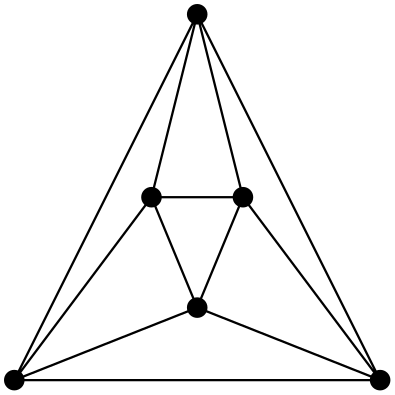
\includegraphics[width=0.16\linewidth]{platonic.png}
\caption{Task 1 graph}
\label{fig:platonic}
\end{figure}

\begin{enumerate}
\item Compute $C(G)$ and $L(G)$ for the graph in Figure~\ref{fig:platonic}.

\item Compute $C(G)$ and $L(G)$ for the wheel graph $W_n$ (a cycle $C_n$ plus one hub adjacent to all cycle vertices).

\item Compute $C(G)$ and $L(G)$ for the complete bipartite graph $K_{n,n}$.

\item Compute $C(G)$ and $L(G)$ for the complete tripartite graph $K_{n,n,n}$.

\item Compute $C(G)$ and $L(G)$ for graph $B_{n,n}$ defined as follows:
\begin{itemize}
\item take two copies of $C_n$,
\item connect the copies with all possible cross edges (a complete bipartite connection).
\end{itemize}

\item Compute $L(G)$ for $K_n \times K_n$ (Cartesian product).

\end{enumerate}

\section*{Diameter and scaling}

Recall the diameter definition:
\[
\operatorname{diam}(G)=\max_{u,v\in V} d(u,v).
\]

\begin{enumerate}[resume]
\item Find the diameter of a square lattice (grid) with $L$ edges per side (equivalently $L+1$ vertices) on each side.

\item Find the diameter of the corresponding $d$-dimensional hypercubic lattice with $L$ edges per side. Express it also as a function of the number of vertices $n$.

\item A Cayley tree has branching factor $k-1$ away from the root. Show that the number of vertices reached exactly at distance $d\ge 1$ from the root is
\[
k(k-1)^{d-1},
\]
then derive an expression for diameter in terms of $k$ and $n$.

\item Let a binary tree (Cayley tree with $k=3$) have $d$ levels and additionally connect sibling leaves on the last level. Compute the clustering coefficient.

\end{enumerate}

\end{document}
